\documentclass[spanish]{beamer}
\usepackage[ansinew]{inputenc} % Acepta caracteres en castellano
\usepackage[spanish]{babel}    % silabea palabras castellanas
\usepackage{amsmath}
\usepackage{mathtools,cancel} % cancela con una flecha \cancelto{0}{XXXX}
\renewcommand{\CancelColor}{\color{red}} %change cancel color to red
\usepackage{amsfonts}
\usepackage{amssymb}
\usepackage{dsfont}
\usepackage{graphicx}
\usepackage{geometry}
\usetheme{Madrid}
\usecolortheme{beaver}
\usepackage{textpos}
% Logo  en el comienzo 
\addtobeamertemplate{frametitle}{}{%
\begin{textblock*}{100mm}(.85\textwidth,-1cm)
{\includegraphics[height=0.4in, keepaspectratio=true]{/Users/luisnunez/Dropbox/MisDocumentos/UIS/UISImagenInstitucional/UISLOGO.png}}
\end{textblock*}}

\begin{document}

\title{\textbf{Vector Laplace-Runge-Lenz} }
\author[L.A. N��ez]{\textbf{Luis A. N��ez}}  
\institute[UIS]{\textit{Escuela de F�sica, Facultad de Ciencias, } \\
\textit{Universidad Industrial de Santander, Santander, Colombia } \\
{\includegraphics[height=0.4in, keepaspectratio=true]{/Users/luisnunez/Dropbox/MisDocumentos/UIS/UISImagenInstitucional/UISLOGO.png}}
}
\date{\today}
\maketitle


\begin{frame}
\frametitle{Agenda}
  \tableofcontents
\end{frame}


%%%%% Diapo 1
\section{El problema de Kepler y el vector $\mathbf{A}$, Laplace-Runge-Lenz }
\frame{
  \frametitle{El vector $\mathbf{A}$}
   \begin{itemize}  
  	\item<1-> La trayectoria del problema de Kepler con el potencial central $V(r)=-k / r$ y la fuerza gravitacional $\mathbf{f}(r)=f(r) \hat{\mathbf{r}}$, con $f(r)=-k / r^2$, es una secci�n c�nica, $\frac{q}{r}=1+e \cos \theta$, donde $q=L^2 / \mu k$, y $e=\sqrt{1+\frac{2 E L^2}{\mu k^2}}$.
	\item<2-> Podemos definir $\mathbf{r} \cdot \mathbf{A}= r A \cos \theta = L^2-\mu k r$, con $A \equiv \mu k e =$ cte.
	\item<3-> $\mathbf{A}$ es un vector de magnitud es constante y direcci�n debe estar en la direcci�n del perihelio. Si la direcci�n est� en el eje $x$,  $\mathbf{A}=\mu k e \hat{\mathbf{i}}$.
	  \begin{figure}[t]
		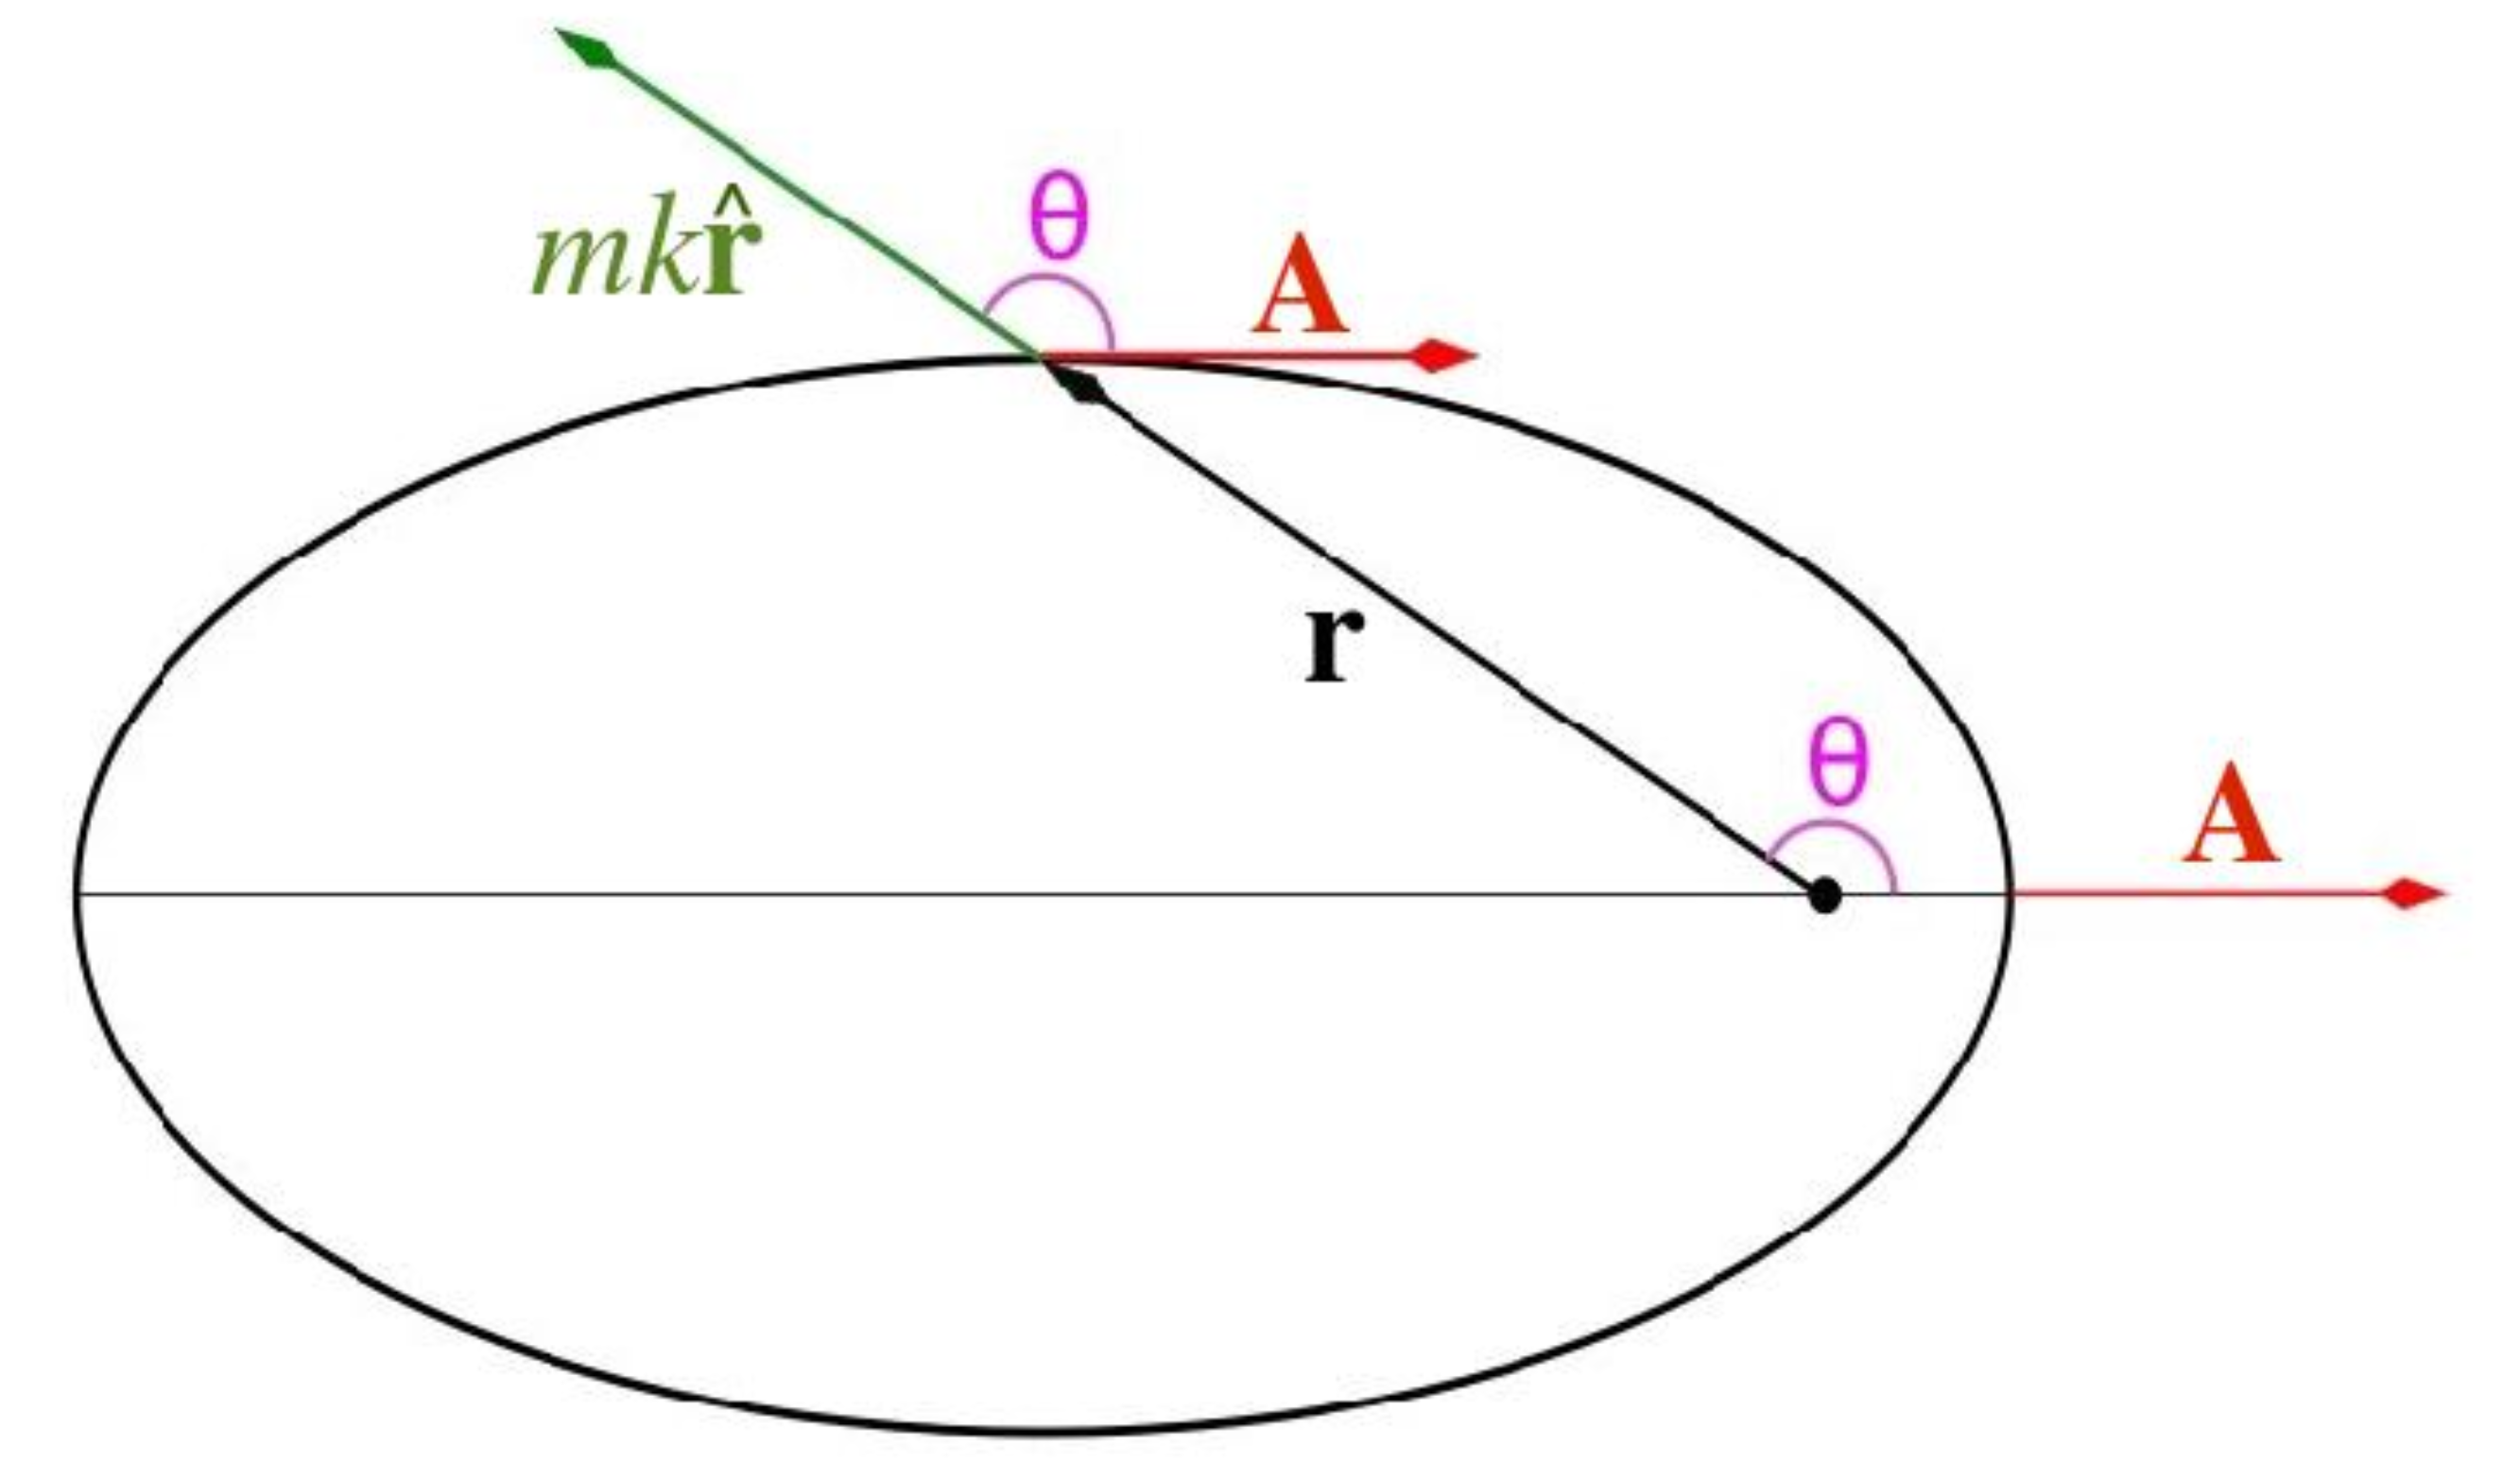
\includegraphics[width=1.8in]{Figuras/VectorA.png}
   	\end{figure}
	\item<4-> Como $L^2=\mathbf{L} \cdot \mathbf{L}=\mathbf{L} \cdot(\mathbf{r} \times \mathbf{p})=\mathbf{r} \cdot(\mathbf{p} \times \mathbf{l}) \Rightarrow \mathbf{r} \cdot \mathbf{A}=\mathbf{r} \cdot[(\mathbf{p} \times \mathbf{L})-\mu k \hat{\mathbf{r}}]$
	\item<5-> Donde $\mathbf{A} \equiv \mathbf{p} \times \mathbf{L} -\mu k \hat{\mathbf{r}}$ y tambi�n $\mathbf{A} \cdot \mathbf{L}=0$
	 
    \end{itemize}
}
%%%%% Diapo 2
\section{El vector $\mathbf{A}$ como cantidad conservada}
\frame{
  \frametitle{$\mathbf{A}$ es cantidad conservada}
   \begin{itemize}  
  	\item<1-> Consideremos $\frac{d \mathbf{A}}{d t}=\frac{d}{d t}(\mathbf{p} \times \mathbf{L})-\mu k \frac{d \hat{\mathbf{r}}}{d t}$
	\item<2-> 
    \end{itemize}
}

%%%%% Diapo 2
\section{Secci�n}
\frame{
  \frametitle{T�tulo transparencia}
   	\begin{itemize}  
  \item<1-> 
    \end{itemize}
}
%%%%% Diapo 2
\section{Secci�n}
\frame{
  \frametitle{T�tulo transparencia}
   	\begin{itemize}  
  \item<1-> 
    \end{itemize}
}
%%%%% Diapo 2
\section{Secci�n}
\frame{
  \frametitle{T�tulo transparencia}
   	\begin{itemize}  
  \item<1-> 
    \end{itemize}
}
%%%%% Diapo 2
\section{Secci�n}
\frame{
  \frametitle{T�tulo transparencia}
   	\begin{itemize}  
  \item<1-> 
    \end{itemize}
}
  
\end{document}
